\chapter{Representational Adequacy: One Geometry, Four Presentations}

\section{Adequacy Made Measurable}

Chapter 7 asked what a picture of a structure can carry, and Chapter 8 asked what a camera does to it. This chapter fixes a single geometry and changes only how it is presented. The development plan of this book states the governing idea as an inequality. Given a full state $x$, a reduced representation $r(x)$, and a question $Q$, a procedure $\widehat Q$ that answers the question from the reduced representation is adequate to the extent that
\[
  d\bigl(Q(x),\,\widehat Q(r(x))\bigr)\le\varepsilon
\]
over a stated domain of states. Here the state $x$ is the geometry of the habitat of Chapter 3, the representation $r$ is a presentation (a plan, an eye-level view, a cutaway, a wireframe), the question $Q$ is a property of the geometry that someone might want to know, and $\widehat Q$ is whatever a reader, or a script standing in for a reader, does with the image. The same presentation can be adequate for one question and badly wrong for another, so no presentation is good in itself, and a statement about a presentation has the form: for this question, on this geometry, with this reading procedure, the error is this large.

The plan is to make the left side of the inequality computable in a few cases, so that the habit of asking the question has numbers to attach to it. Two cautions apply. A reading procedure must be specified before the error can be measured, and a human reader's procedure is not fully specified, so the procedures used here are simple automatic ones whose failures are informative but not exhaustive. And $\varepsilon$ comes from the purpose of the work, not from the measurement: whether an error of $8$ percentage points in a visible-floor fraction matters depends on what the fraction will be used for.

\section{The Habitat as Data}

The habitat of Chapter 3 was built by hand from dimensions in the text. To measure anything about it, the same construction is needed as data. The script below builds it in a collection named \texttt{Habitat}, with the platform top at $z=0$, the north wall $6$ long, the east and west walls $5.6$ long between the inner faces of the north and south boundaries, a south wall in two blocks that leave a gap, and a low plinth. There is no roof. Two entrance variants stand for the two saved files of Exercise 3.4: a gap of width $1.2$ centred on the south wall, and a gap of the same width at the east end, $x\in[1.6,2.8]$. The plinth is $0.8\times0.8\times0.5$ at $(-1,1)$ in both.

\Needspace{26\baselineskip}
\lstinputlisting[language=Python,basicstyle=\ttfamily\footnotesize,breaklines=true,frame=single,columns=fullflexible,keepspaces=true,firstline=12,lastline=45]{habitat.py}

The script was run in Blender 5.2.2 and its check function read the built objects back. Each variant has seven objects; the platform top is at $z=0.000$; every wall spans $z=0$ to $2.5$; the south gap measures $1.200$ in both variants; the east wall lies between $x=2.8$ and $3.0$ and has length $5.60$; and the inner faces of the north and south walls are at $y=2.80$ and $y=-2.80$, where the ends of the east and west walls stop. The construction is therefore the one the chapter describes, and the numbers below refer to it.

\section{Two Questions}

Two questions about this geometry are used throughout. Question A concerns an observer and has the form of Exercise 3.4: what fraction of the interior floor can a person standing in the doorway, with eyes at height $1.6$, see? Question B concerns the structure: where is the entrance?

The answer to A is defined by ray-casting. The interior floor, $5.6\times5.6$, is divided into $56\times56$ cells of side $0.1$. A cell counts as reachable if the straight segment from the eye, placed in the plane of the south wall at the centre of the gap, to the cell centre meets no object. For the centred entrance $2806$ of $3136$ cells are reachable, $89.5$ percent. For the east entrance $2646$ are reachable, $84.4$ percent. The two variants differ by five percentage points. Two things are expected to contribute, the thickness of the wall beside the doorway, which hides a strip of floor along the south wall, and the position of the observer, who stands near a corner in the second variant; the contribution of each was not separated here. The plinth hides a shadow-shaped region behind it in both. The truth for B is the gap, $[-0.6,0.6]$ or $[1.6,2.8]$.

\section{Four Presentations}

Figure 9.1 shows the east-entrance habitat in four presentations: a plan, an eye-level view from the doorway, a cutaway, and a wireframe. The geometry is identical in all four and the lighting is ambient only, so no cast shadow decides what a panel appears to show.

\begin{figure}[ht]
\centering
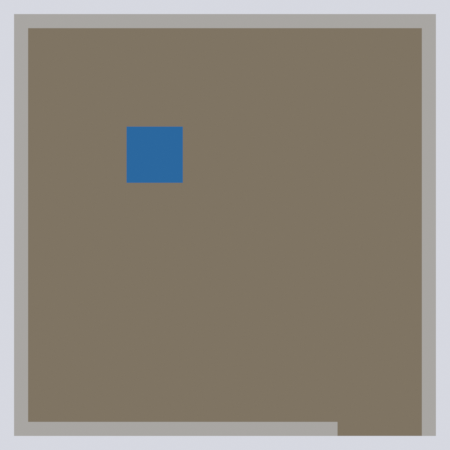
\includegraphics[width=0.48\textwidth]{figs/fig9_plan.png}\hfill
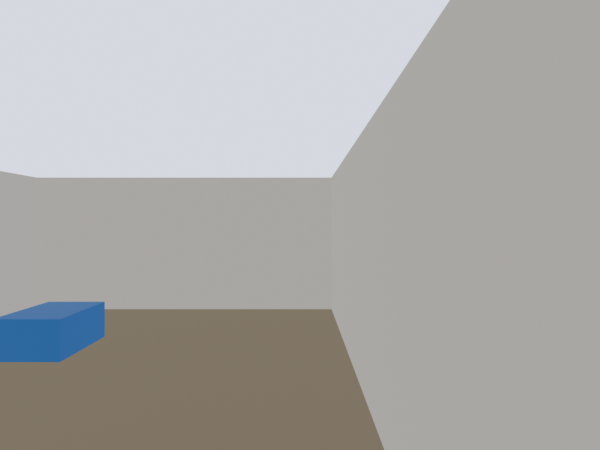
\includegraphics[width=0.48\textwidth]{figs/fig9_eye.png}\\[4pt]
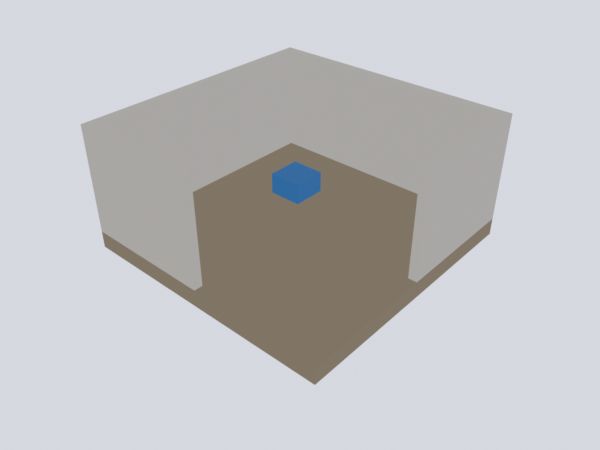
\includegraphics[width=0.48\textwidth]{figs/fig9_cut.png}\hfill
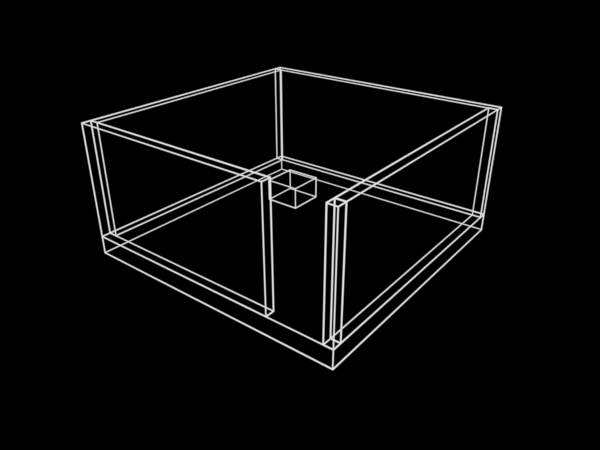
\includegraphics[width=0.48\textwidth]{figs/fig9_wire.png}
\caption{The east-entrance habitat. Top left, plan from above with an orthographic camera. Top right, eye-level view at $1.6$ from the doorway, $90^\circ$ horizontal field of view, looking north. Bottom left, a cutaway made with a Boolean difference that removes the south-east quadrant of the walls. Bottom right, the same geometry as a wireframe from the oblique camera used for the counts in the text.}
\end{figure}

\paragraph{Plan.} The plan answers Question B well. The wall tops, floor, and plinth top are flat colours, and reading the gap as the run of non-wall pixels along the south wall recovered its ends to within one pixel at every resolution tried.

\begin{center}
\begin{tabular}{rrrr}
\toprule
Size & mm per pixel & Error, centre & Error, east\\
\midrule
100 px & 64 & 24 mm & 16 mm\\
200 px & 32 & 8 mm & 16 mm\\
400 px & 16 & 8 mm & 0 mm\\
\bottomrule
\end{tabular}
\end{center}

The same plan answers Question A badly. Every point of the floor is visible from above except the footprint of the plinth, so the share of floor-coloured pixels in the interior, which is the only answer the plan can give, was $97.8$, $97.4$, and $97.96$ percent at the three resolutions, against a geometric value of $1-0.64/31.36=97.96$ percent. The plan reports $98$ percent where the truth is $89.5$ or $84.4$. The error is about $8.5$ points in one variant and $13.5$ in the other, and the plan reports the same number for the two entrances. The reason is structural: the plan is the view of an observer at infinity above the room, and Question A asks about an observer in a doorway. A plan that is accurate and well rendered is not adequate to the question.

\paragraph{Eye-level view.} The eye-level view is the observer's own sample, and it can be made to answer A by a rendering trick. The floor is given an emission colour that encodes its position, red proportional to $x$ and green to $y$, and everything else is black, with anti-aliasing off, a single sample, and a raw view transform so that the stored values are the assigned values. Each floor pixel then says which floor point it shows, and the cells that appear are the cells the image can speak about. The script \texttt{presentations.py} did this at $800\times600$ with a $90^\circ$ lens. For the centred entrance the image contained $1745$ distinct cells, and $1724$ of them were exactly the cells that the ray-cast found both reachable and inside the frame; for the east entrance the image held $1307$ cells, of which $1294$ matched. No cell that was reachable and in frame was missing from the image. The $21$ and $13$ extra cells are cells whose centres are hidden but whose edges are visible, which is the centre-versus-surface distinction of Chapter 7 in a different setting.

The eye-level view has a different limit. A $90^\circ$ frame cannot contain what is beside or behind the observer, and of the $2806$ and $2646$ reachable cells, $1082$ and $1352$ lay outside the frame. The image therefore speaks to $1724/2806=61$ percent of what the observer can see in the first variant and $1294/2646=49$ percent in the second. The fraction of the floor visible within the frame was $55.0$ and $41.3$ percent, and that number is a property of the camera's field of view as much as of the room. Question A as posed asks for the observer's visibility, and a single narrow-angle image underestimates it. A panoramic camera or several views turned in different directions would answer it, and the cost, as in Chapter 8, is a count of views.

\paragraph{Cutaway.} A cutaway shows interior arrangement by removing the near surfaces, and what it removes cannot be read from it. The cutter used here deletes the south-east quadrant of the walls, which contains the entrance of the east variant, so the cutaway shows the plinth and the north and west walls clearly and shows neither the entrance nor the walls that determine what the doorway observer sees. For Question A it cannot be used at all, since the walls that hide the floor from the doorway are among those removed. For Question B it answers wrongly in a particular way: the opening where the south wall has been cut away looks like an entrance of great width, and nothing in the image distinguishes the cut from the doorway. A cutaway is adequate for questions about what the removed surfaces were hiding, and a reader needs to be told what was removed.

\paragraph{Wireframe.} A wireframe preserves all the edges, hidden or not, and so keeps the geometry's incidence structure while discarding surfaces. What it adds is crossings that are not in the geometry. Using the oblique camera of the figure, with $84$ edges in the seven meshes, $82$ pairs of edges cross on the screen without meeting in space and $7$ cross where they also meet, for the centred entrance, and $62$ and $7$ for the east entrance. The false crossings are about ten times as many as the true ones. If only the edges whose midpoints are unobstructed are drawn, a crude stand-in for a solid view, the false crossings fall to $8$ and $3$ with $3$ true ones. From an elevation straight toward the south wall the wireframe has $74$ and $58$ false crossings and none true, because the edges of the near and far walls project onto each other. A reader looking at a wireframe has to decide, at each crossing, whether two edges meet, and the numbers say how often the picture offers that decision as a trap. The measure counts crossings of edges and does not count overlapping collinear edges, which also confuse a reader, so it understates the problem.

\section{What the Experiment Does Not Show}

The experiment used one geometry in two variants and one observer height, and the questions were chosen because they separate the presentations. Nothing here shows that a plan is a poor presentation in general or that a wireframe is poor; they answer different questions, and the reader who wants to know where the entrance is should consult the plan. The reading procedures were automatic: the cell-identity decoding is not how a person looks at a picture, and a person might use cues the procedure ignores, such as the convergence of lines to read depth in the eye-level view. The measurement of false wireframe crossings assumes that every crossing is a risk of misreading, which a practised reader may resolve at a glance. The distance used, an absolute difference in a fraction or a position, is one of many that could stand for $d$ in the adequacy inequality. And the tolerance $\varepsilon$ was never specified, because it is a matter of purpose. The purpose of the habitat in this book is to be revisited from several positions, which makes Question A the more relevant of the two, and makes the plan, despite its excellent recovery of the entrance, the least adequate presentation for it.

\section{Writing an Adequacy Statement}

A caption or a report that uses a presentation can state its adequacy compactly, in the form the inequality suggests. The statement names the geometry, the question, the presentation, the reading procedure, the distance, and the measured error. For the habitat it can read: \emph{for the east-entrance habitat, the question of what fraction of the floor is visible from the doorway at height $1.6$, read as the share of floor-coloured pixels in the plan, has an error of $13.5$ percentage points, so the plan is not used for it; read from a cell-identity render at $90^\circ$ field of view, the image covers $49$ percent of the reachable cells, so a single image underestimates visibility.} The sentence is longer than a caption usually is, and it can be shortened once the structure is understood. What must not be shortened away is the question, since the same image supports a different statement for each question.

\begin{exercise}[9.1: Move the observer]
Repeat Question A for an observer standing $1.0$ inside the room at the centre of the gap, and for an observer seated with eye height $1.1$. Report the reachable fraction for both entrance variants and describe which of the four presentations of Figure 9.1 changes its answer, and which does not.
\end{exercise}

\begin{exercise}[9.2: A cutaway that answers]
Choose a cutter that removes only the roofless wall above eye height $1.6$ on the east side and keeps the south wall intact. State one question that this cutaway answers and one that it does not, and test each with a reading procedure of your own.
\end{exercise}

\begin{exercise}[9.3: A panoramic answer]
Use a panoramic camera, or four views turned by $90^\circ$ about the vertical axis at the doorway, to answer Question A from images alone. Report the number of cells the images can speak to and compare it with the ray-cast truth. State the number of views and the field of view that reached at least $95$ percent of the reachable cells.
\end{exercise}

\begin{exercise}[9.4: Moving the plinth]
Move the plinth to the middle of the room and repeat the ray-cast truth for Question A. Predict beforehand whether the reachable fraction will rise or fall, state the geometric reason, and then measure.
\end{exercise}
